\chapter{Partenariat Automne\&Détente}
\section{Déclarer une activité PAD (DA)}
Pour déclarer une activité de Partenariat Automne Détente, dans le volet de navigation de gauche, développez le volet "Partenariat Aut. \& Dét."  Cliquez ensuite sur l'entrée "Activités". La liste de vos activités déclarées s'affiche.

\medskip

\begin{center}
\begin{tabular}{|c|c|c|c|c|c|c|}
\hline
Numéro de dossier & Type & Congé & Période & Dénomination & Partenariat & Commune\\
  \hline
& & & & & &\\
  \hline
\end{tabular}
\end{center}
\smallskip



\begin{itemize}
    \item \textbf{N° de dossier}; 
    \item \textbf{Type d'activité}: résidentielle (\textit{plaine}) ou non-résidentielle (\textit{séjour ou camp});
    \item \textbf{Congés}: Automne ou Détente;
    \item \textbf{Période}: les dates de votre activité;
    \item \textbf{Dénomination}: le nom de votre activité;
    \item \textbf{Partenariat}: le nom du partenariat; 
    \item \textbf{Commune}: la commune où se déroulera l'activité.
\end{itemize}

Pour déclarer une activité, cliquez sur \ovalbox{Déclarer une activité}. Vous serez invité à compléter les données de l'activité et du partenariat. 

\begin{figure}[ht!]
    \centering
    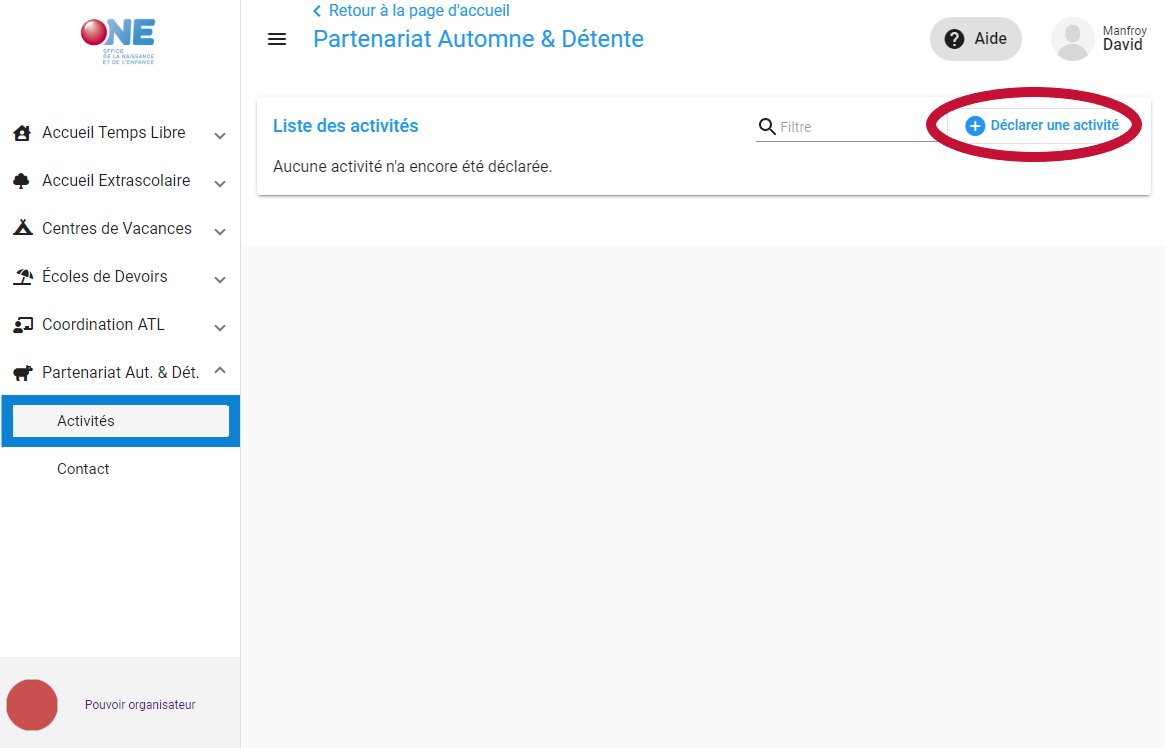
\includegraphics[width=12cm]{Images/pad/liste-acti.png}
    \caption{Liste des activités de partenariat et bouton de déclaration}
    \label{fig:pad_liste}
\end{figure}


\subsection{DA (1/4) - Caractéristiques}

\begin{figure}[ht!]
    \centering
    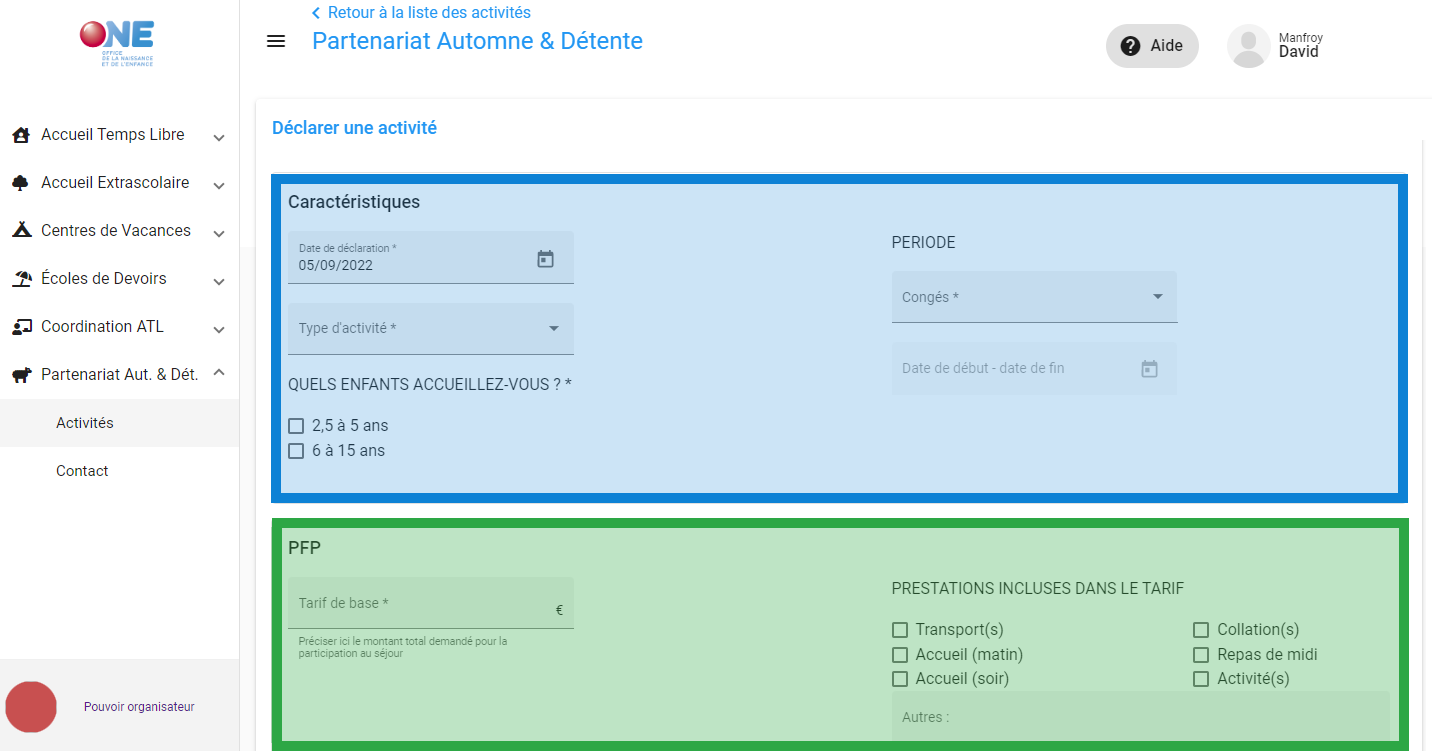
\includegraphics[width=13cm]{Images/pad/da1.png}
    \caption{Cadre de déclaration (caractéristiques et PFP)}
    \label{fig:pad_da1}
\end{figure}

La date de déclaration sera celle de la date du jour. Choisissez le type d'activité : \textbf{Résidentielle} ou \textbf{Non-résidentielle}. Renseignez la période de congé, ainsi que les dates de début et de fin de vos activités. Sélectionnez la ou les tranches d'âge des enfants accueillis en cochant la ou les cases adéquates. (Voir en bleu dans la figure \ref{fig:pad_da1}).



\subsection{DA (2/4) - Participation aux frais (PFP)}
Mentionnez le "tarif de base" de participation demandé aux parents. Si vous avez différents tarifs, renseignez celui qui est le plus haut.

En fonction du type d'activité, vous devez renseigner les prestations qui sont incluses dans la PFP. Un champ 'Autre' vous permet d'ajouter des éléments supplémentaires. (Voir en vert dans la figure \ref{fig:pad_da1}). 


\subsection{DA (3/4) - Lieu}
\begin{figure}[h!]
    \centering
    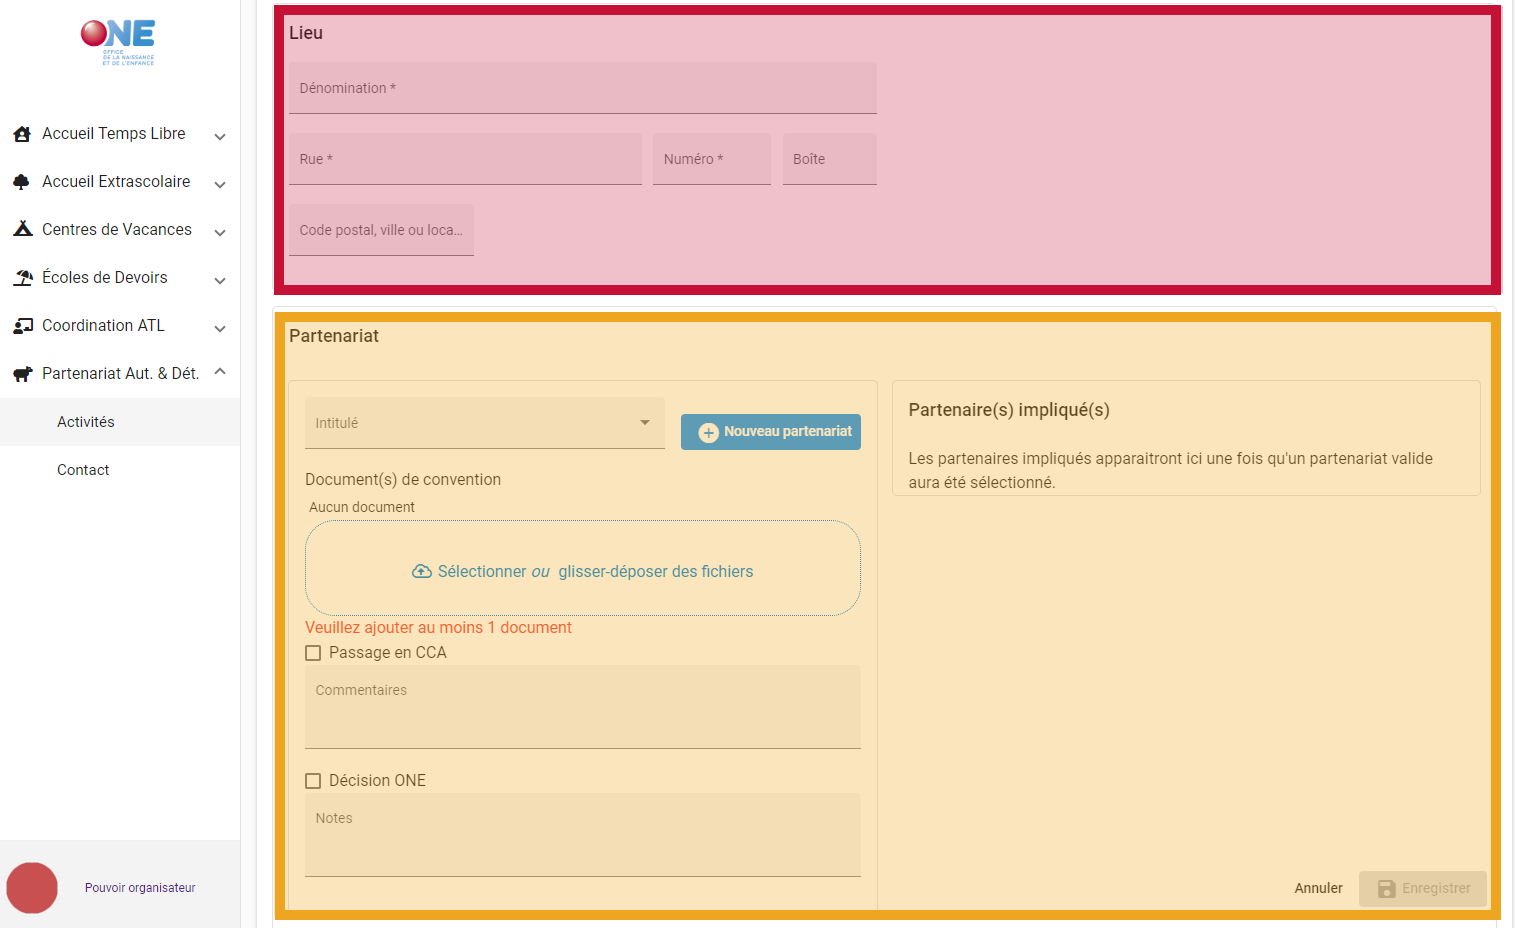
\includegraphics[width=13cm]{Images/pad/da2.png}
    \caption{Cadre de déclaration (Lieu et Partenariat)}
    \label{fig:pad_da2}
\end{figure}
Renseignez une dénomination pour votre activité. Cette dénomination est un champ libre. Il peut s'agir de la thématique de votre activité, du lieu, du nom que vous communiquez aux parents, etc.  Indiquez ensuite l'adresse de l'activité. (Voir en rouge dans la figure \ref{fig:pad_da2}). 

\subsection{DA (4/4) - Partenariat}
Les partenariats concernent votre organisation et un ou plusieurs autres organismes. Ces autres organismes peuvent ou non être reconnus par l'ONE ou par une autre institution (secteur culturel, secteur de l'enfance, secteur sportif, ...). (Voir en orange dans la figure \ref{fig:pad_da2}). 


\subsubsection{Création d'un partenariat}
Cliquez sur \ovalbox{+ Nouveau partenariat}. La fenêtre de création de partenariat s'ouvre. 

\begin{figure}[h!]
    \centering
    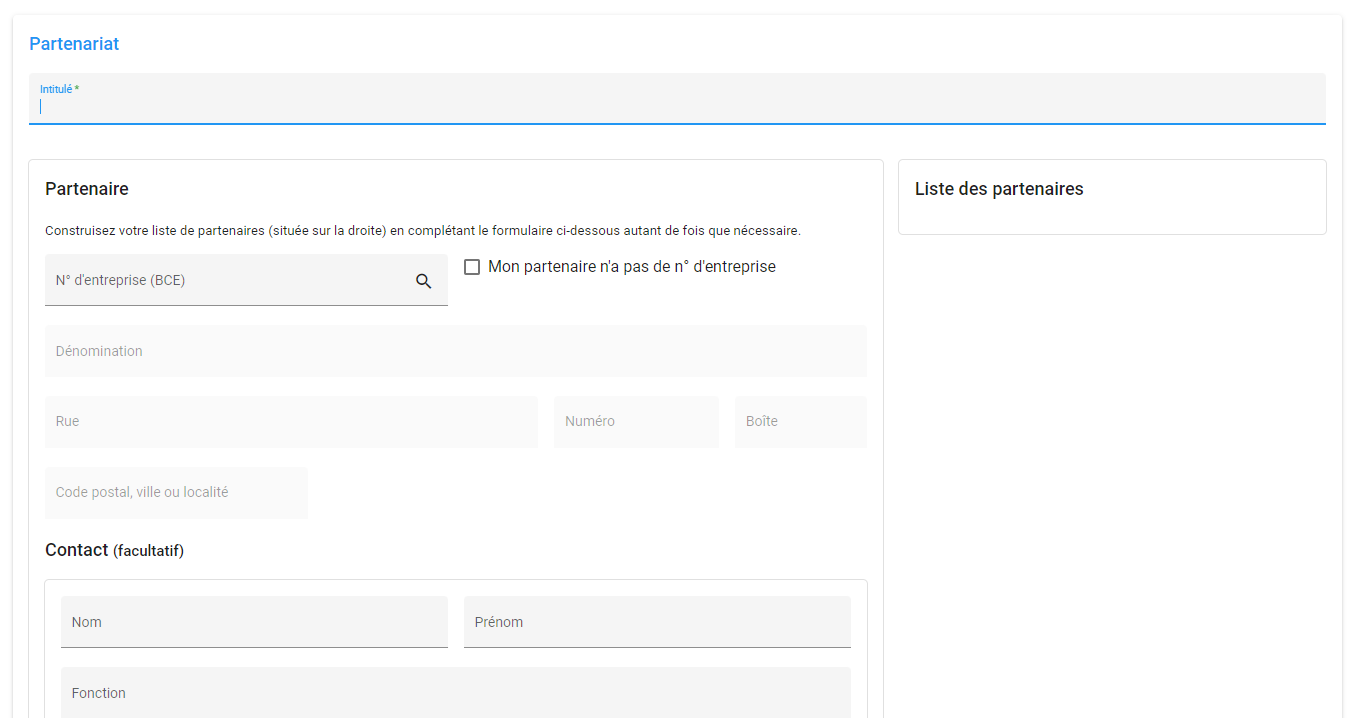
\includegraphics[width=11cm]{Images/pad/new-partenariat.png}
    \caption{Création d'un nouveau partenariat}
    \label{fig:pad_da_nouveau_partenariat}
\end{figure}



\begin{itemize}
    \item \textbf{Intitulé}: spécifiez l'intitulé du Partenariat. Il s'agit du nom que vous donnez à votre partenariat.
    \item \textbf{Partenaire}: ajoutez le numéro d'entreprise de l'organisme partenaire. Cliquez ensuite sur la petite loupe. Le Portail Pro ira chercher les informations dans la Banque Carrefour des Entreprises et affichera la dénomination officielle et l'adresse du siège social. Si le partenaire est une association de fait, cochez la case attenante et complétez soigneusement les données.
    \item \textbf{Contact}: les coordonnées de la personne de contact de l'organisme partenaire. 
\end{itemize}


Une fois ces données complétées, cliquez sur \ovalbox{Ajouter le partenaire}. Le partenaire est alors enregistré pour ce partenariat. Réalisez cette opération pour chacun des partenaires qui font partie de ce partenariat.

La liste des partenaires enregistrés pour le partenariat est affichée dans "Liste des partenaires". 

Lorsque tous les partenaires ont été enregistrés, cliquez sur \ovalbox{Créer le partenariat}.


\subsubsection{Sélection d'un partenariat}
Sélectionnez dans la liste déroulante "intitulé", le partenariat concerné par l'activité. La liste vous proposera les partenariats qui ont été créés à l'étape précédente.

\subsubsection{Chargement de la convention}
Une copie de la convention signée entre les différentes parties prenantes doit être chargée. Cliquez sur le petit nuage afin de charger la pièce demandée.



\subsubsection{Passage en CCA}
Le partenariat doit avoir été approuvé en Commission communale de l'accueil. En cochant la case "Passage en CCA", vous confirmez que la CCA s'est positionnée favorablement à l'établissement du partenariat et à l'organisation de l'activité. 

Un champ commentaire est disponible pour ajouter tout complément d'informations utiles pour l'ONE.


\begin{remarque} %Cas particulier des communes sans CLE
Si la commune n'a pas de Programme CLE (coordination locale pour l'enfance), vous pouvez déclarer sans cocher la case. Dans ce cas, c'est l'ONE qui décidera d'approuver votre projet de partenariat.
\end{remarque}

\section{Demander des subsides pour une activité PAD (DS)}

Pour envoyer une demande de subsides, il est nécessaire de compléter entièrement les deux onglets suivants: \ovalbox{Encadrement} et \ovalbox{Présences}.

%\vspace*{4mm}
%\centerline{
\includegraphics[width=18cm]{Images/cdv/cdv-onglets-ds.png}}

\subsection{DS (1/3) - L'onglet "Encadrement"}\label{encadrementpad}



Cet onglet reprend le personnel d'encadrement qui preste pour votre activité de partenariat (fig. \ref{fig:pad_encadrement}). Vous renseignerez les responsables et les animateurs qui ont animé les enfants. Pour chacun d'eux, vous pourrez renseigner leur fonction (responsable ou animateur), leur statut (contractuel ou volontaire) et les qualifications pour leur fonction (qualifié ou non qualifié).

\subsubsection{Prestation, qualification ou suppression}
Quelques boutons d'action sont disponibles (fig. \ref{fig:pad_encadrement}):

\begin{figure}[h!]
    \centering
    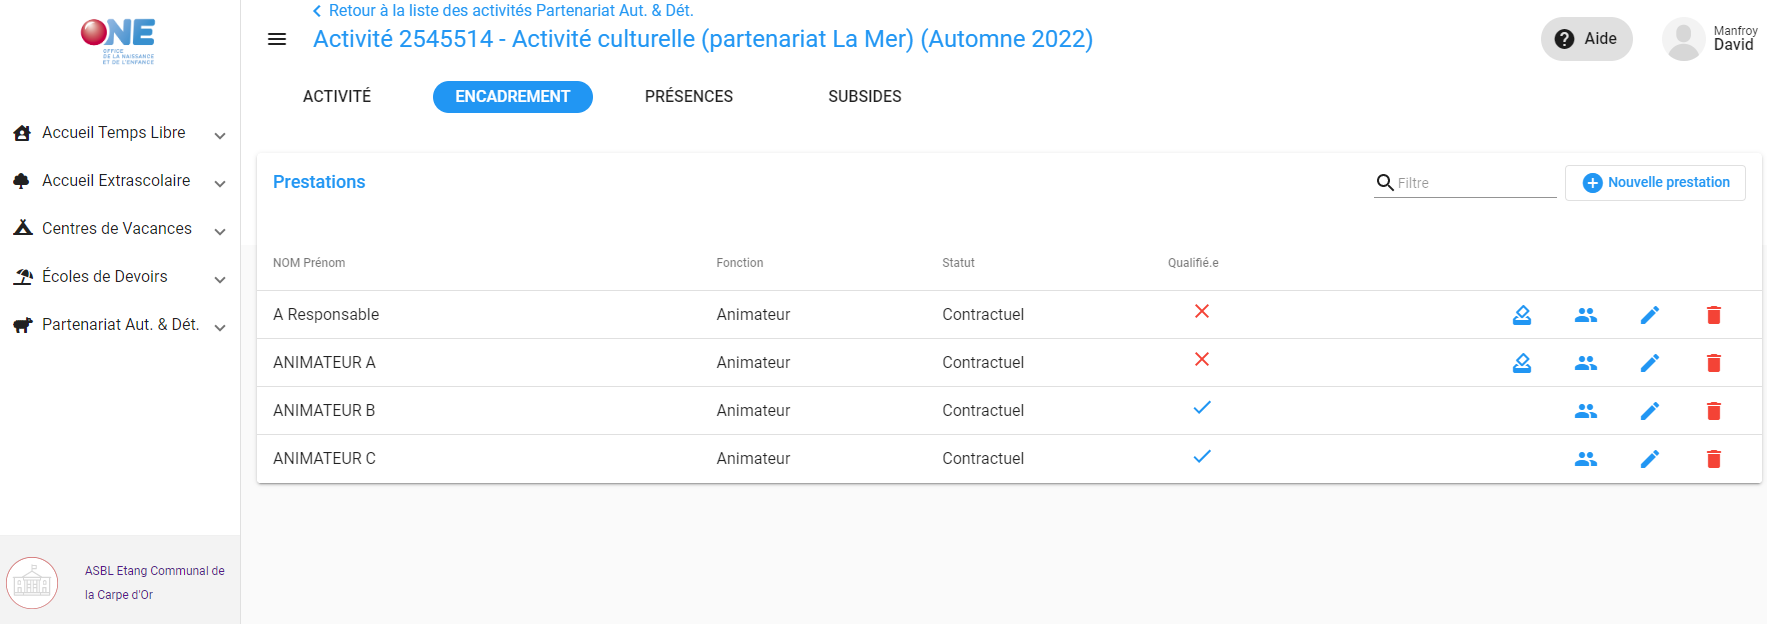
\includegraphics[width=15cm]{Images/pad/onglet-encadrement.png}
    \caption{Onglet encadrement: liste du personnel qui preste pour l'activité}
    \label{fig:pad_encadrement}
\end{figure}

\begin{itemize}
    \item Les \textbf{qualifications} peuvent être renseignées en cliquant sur l'icône 
\includegraphics[width=0.3cm]{Images/icon/button_dmd_qualif.png}.
    \item Les informations de \textbf{prestation} (fonction et statut) sont modifiables en cliquant sur 
\includegraphics[width=0.3cm]{Images/icon/button_modif.png}.
    \item Vous avez également la possibilité de \textbf{supprimer la prestation} en cliquant sur 
\includegraphics[width=0.3cm]{Images/icon/button_poubelle.png}. Celle-ci n'apparaîtra alors plus dans le personnel de votre activité et les données de présences seront supprimées (onglet présences).
\end{itemize} 


%\vspace*{4mm}
%\centerline{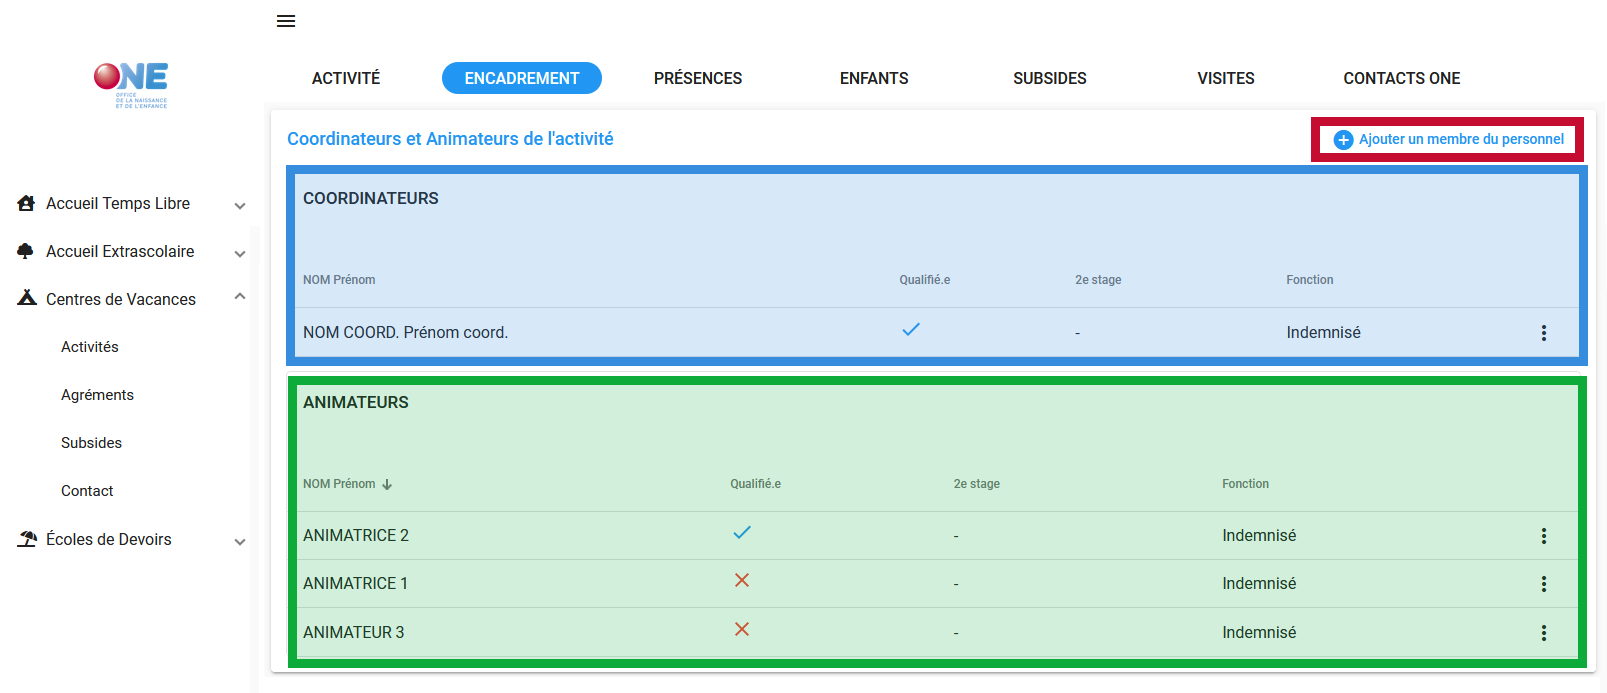
\includegraphics[width=18cm]{Images/cdv/cdv-ds-encadrants.png}}



\subsubsection{Ajouter un membre du personnel}
Cliquez sur \ovalbox{Ajouter une prestation} en haut à droite. Dans l'encadré \fbox{\textbf{Nouvelle prestation}} (fig. \ref{fig:pad_new_prestation}), vous serez invité à ajouter l'encadrant, à indiquer le contexte de sa prestation (contrat de travail, étudiant, stage ou convention de volontariat par exemple), sa fonction et son statut. 

\begin{figure}[h]
    \centering
    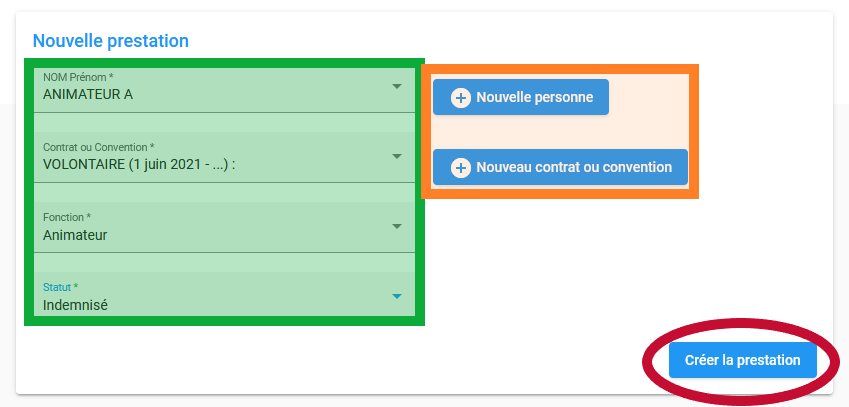
\includegraphics[width=10cm]{Images/cdv/new_prestation.png}
    \caption{Cadre "Nouvelle prestation"}
    \label{fig:pad_new_prestation}
\end{figure}


\begin{enumerate}
    \item En cliquant sur "\textbf{prénom nom}*", vous aurez accès à la liste des personnes qui ont déjà travaillé pour votre pouvoir organisateur; sélectionnez ensuite la personne dans la liste. Si par contre, la personne ne figure pas dans la liste, cliquez sur \ovalbox{Ajouter une personne}. 
    
    \item En cliquant sur "\textbf{Contrat et convention}", la liste vous donnera l'ensemble des liens (contractuels ou conventionnels) que la personne entretient avec votre pouvoir organisateur. Si le contrat n'apparaît pas, vous pouvez cliquer sur \ovalbox{Nouveau contrat/convention}. 
    
    
    
    \item Sélectionnez la \textbf{fonction}: animateur ou coordinateur. 
        \begin{attention}
         Si la personne anime un jour et coordonne le centre un autre jour, il sera nécessaire de l'encoder deux fois. La personne ne pourra pas détenir les deux fonctions pour un même jour (il anime ou il coordonne, mais pas les deux au même moment), il peut, par contre, coordonner un jour et animer un autre jour.
        \end{attention}
    
    
\item Indiquez le \textbf{statut de la personne}: indemnisé ou volontaire. Ces champs seront pré-remplis en fonction du point 2 (contrat et convention), mais peuvent être modifiés. 
\item Cliquez enfin sur \ovalbox{Créer la prestation}. La personne sera alors ajoutée à la liste des encadrants de votre activité.
\end{enumerate}



\subsubsection{Consulter les qualifications de la personne}

Dans l'encadré \textcolor{vert}{vert} de la fig. \ref{fig:pad_encadrement}, vous pouvez voir les qualifications de la personne reconnues par l'ONE:

\begin{itemize}
    \item [$\bullet$]\textbf{\textcolor{bleu}{V}}: la personne est qualifiée pour exercer sa fonction d'animation ou de coordination. 
    \item [$\bullet$]\textbf{\textcolor{rouge}{X}}: la personne n'est pas qualifiée pour exercer sa fonction d'animation ou de coordination. 
    \item [$\bullet$]
\includegraphics[width=0.3cm]{Images/icon/icon_sablier.png}: une demande de qualification est en cours d'analyse auprès de l'ONE. 
    \item [$\bullet$]
\includegraphics[width=0.4cm]{Images/icon/icon_attention.png}: la personne a obtenu sa qualification durant l'année en cours. En fonction de la date d'octroi de la qualification, le calcul de subventionnement peut être impacté. En effet, la personne est considérée comme non qualifiée avant cette date. 
\end{itemize}
\vspace*{3mm}


\subsubsection{Envoyer une demande de qualifications}
\begin{itemize}
    \item Cliquez sur 
\includegraphics[width=0.3cm]{Images/icon/button_dmd_qualif.png}. Vous pourrez alors renseigner les preuves de qualification de la personne.
        \begin{conseil}
        Suivez le point \ref{sec:qualif_person} de ce Guide pour faire une demande de qualification (Mon Équipe). 
        \end{conseil}
    \item Une fois la demande de qualification envoyée dans "Mon Equipe", vous pourrez revenir à la gestion de vos encadrants en cliquant sur le petit encadré jaune "Retourner vers la liste des prestations" situé en bas à droite de votre écran. 
\end{itemize}

 
\subsection{DS (2/3) - L'onglet "Présences"}\label{pad_présence}
Encodez le nombre d'enfants ayant fréquenté votre activité. Complétez également le nombre d'enfants inscrits dont la frais ont été pris en charge par un tiers-payant.

La grille de présences reprend les \textcolor{vert}{dates déclarées} de l'activité de partenariat, les différentes \textcolor{bleu}{tranches d'âge d'enfants} accueillis et votre \textcolor{ocre}{personnel d'encadrement} (voir fig.\ref{fig:pad_encadrement}).

\begin{figure}[h!]
    \centering
    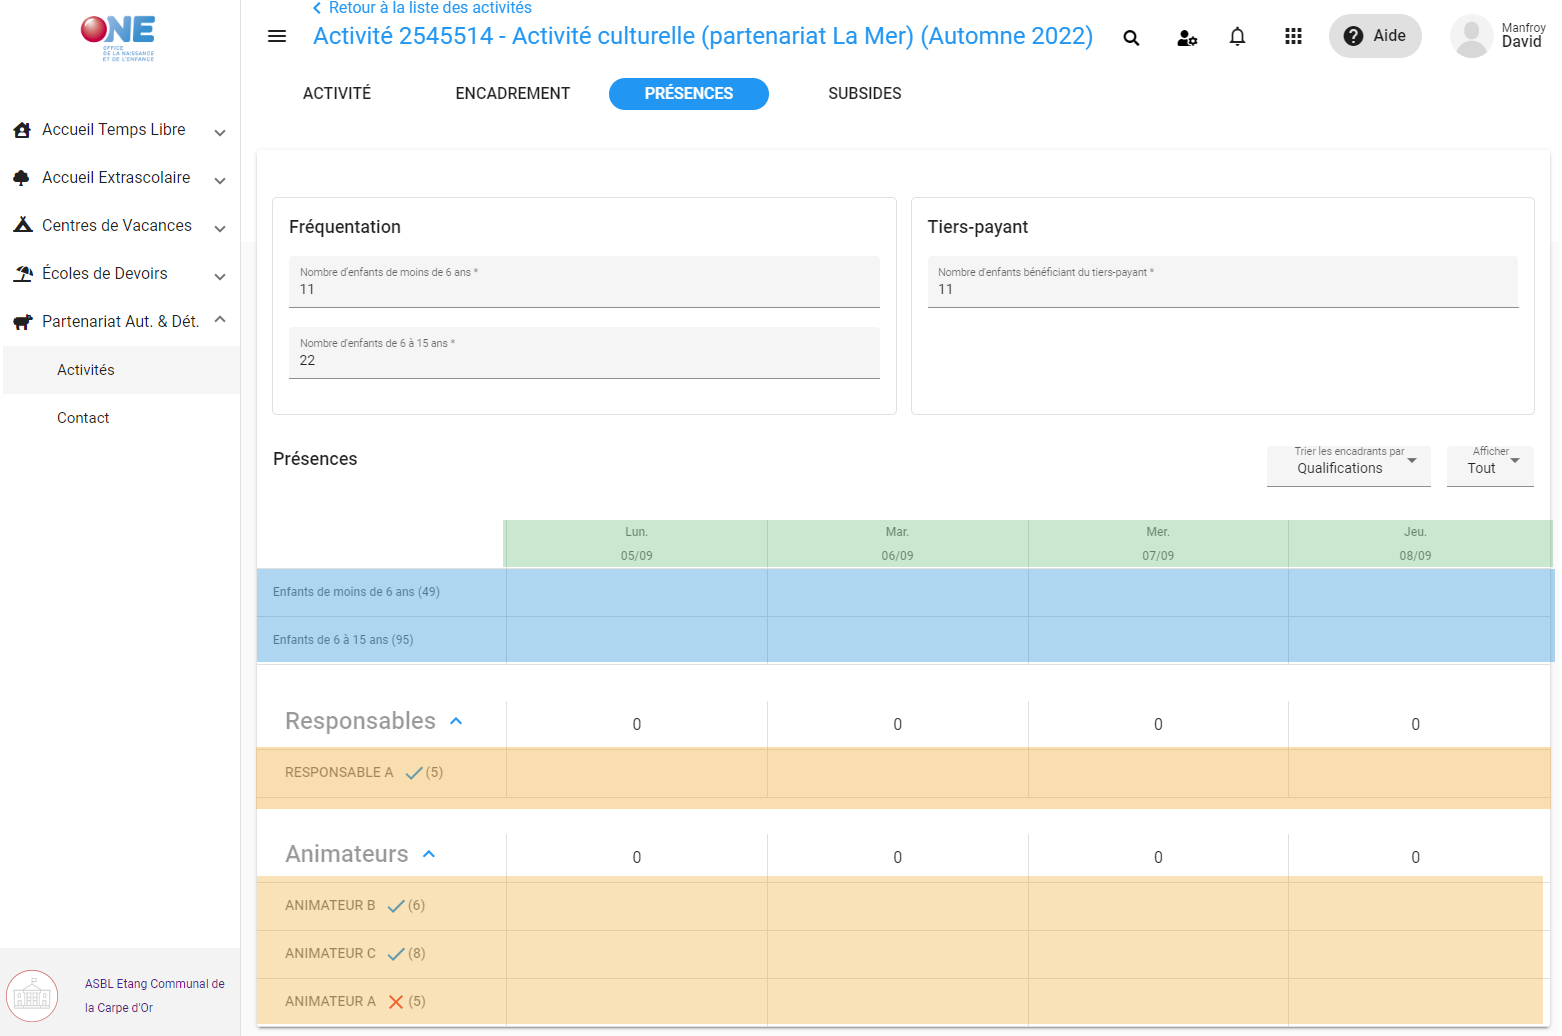
\includegraphics[width=15cm]{Images/pad/onglet-encadrement2.png}
    \caption{Dans l'onglet présence, la grille de présence rependra les dates de votre déclaration d'activité. S'il manque des jours, contactez votre gestionnaire pour qu'il puisse mettre à jour les dates de votre activité de partenariat.}
    \label{fig:pad_presences}
\end{figure}


\subsubsection{Présences des enfants}
\underline{Il y a deux groupes d'âge pour les enfants:}

\begin{itemize}
    \item \textbf{Les moins de six ans}: reprend les enfants de 30 mois à 5 ans;
    \item \textbf{Les plus de six ans}: reprend les enfants de 6 à 15 ans.
\end{itemize}

\subsubsection{Présences des encadrants}
Le personnel repris dans l'onglet \ovalbox{Encadrement} est repris par fonction (coordinateur ou animateur). Pour ajouter un membre du personnel, référez-vous au point \hyperref[encadrementpad]{"DS (1/3) ‐ L’onglet Encadrement"} (\ref{encadrementpad} du guide).

\begin{tcolorbox}[title=Comment encoder les présences des encadrants ?]
Cliquez sur la case du jour pour confirmer que la personne était bien présente. Un petit {\color{bleu}V} apparaîtra. Si une personne a été encodée pour deux fonctions (animateur - coordinateur), elle apparaîtra une première fois dans la section "coordinateur" et une deuxième fois dans "animateur"; par contre, elle ne peut endosser qu'un rôle pour un même jour. 
\end{tcolorbox}


\subsection{DS (3/3) - L'onglet Subsides}
Lorsque les onglets \ovalbox{Encadrement} et \ovalbox{Présences} ont été complètement remplis, vous pouvez procéder à l'envoi de la demande de subsides. Cochez les cases "attestation sur l'honneur" et cliquez ensuite sur \ovalbox{Envoyer ma demande de subsides} (voir fig.\ref{fig:pad_subsides}). 

\begin{figure}[h!]
    \centering
    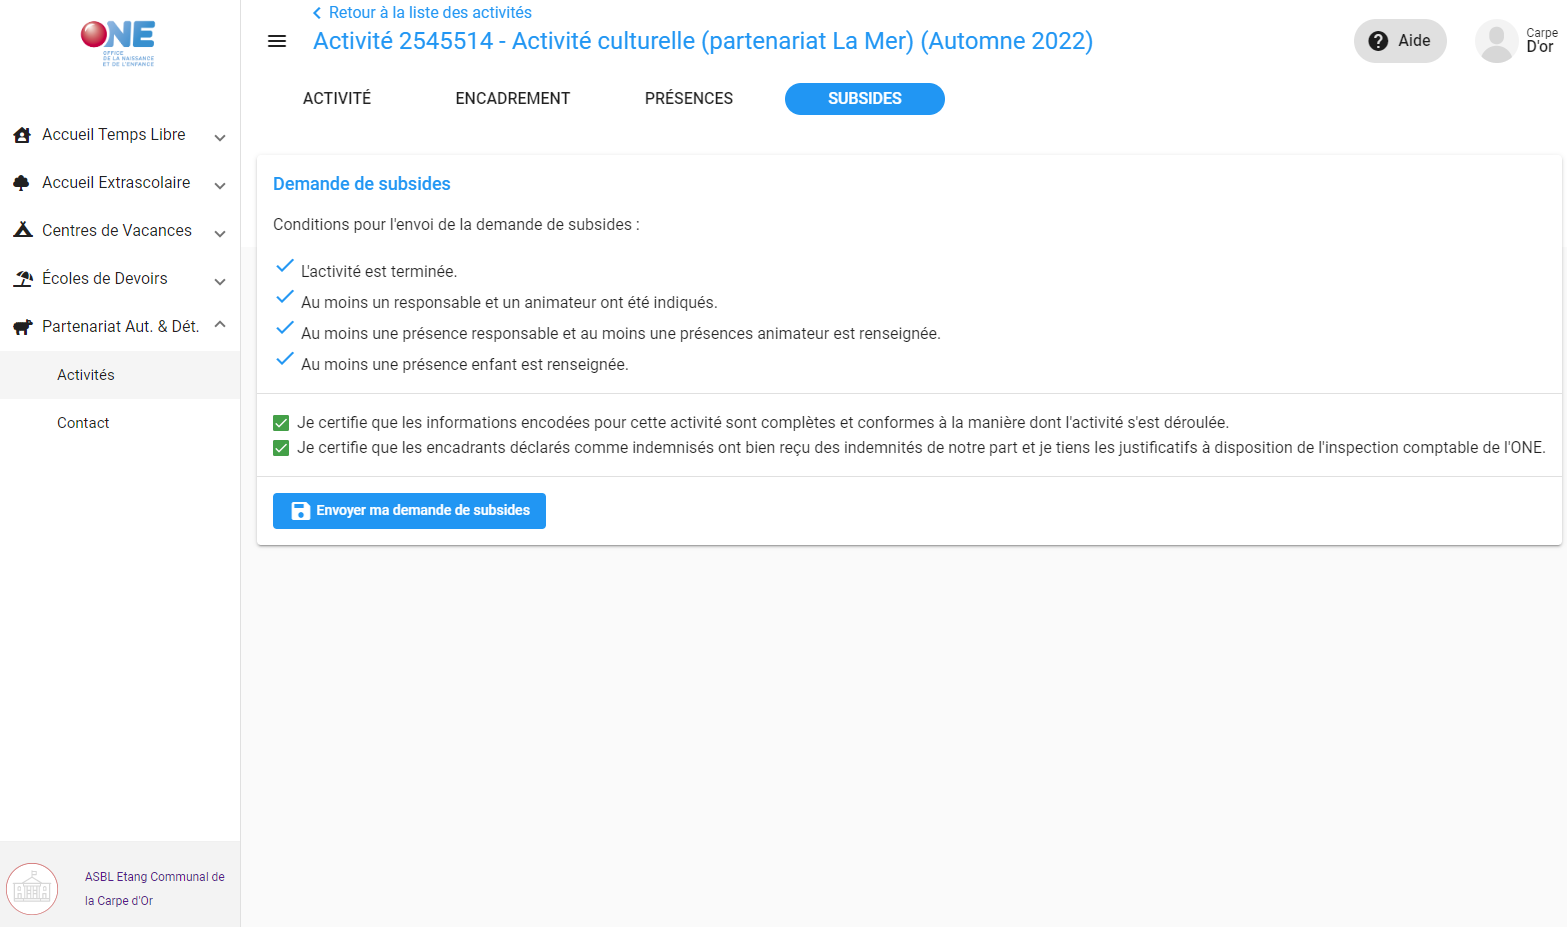
\includegraphics[width=15.5cm]{Images/pad/onglet-subsides.png}
    \caption{L'onglet subsides vous permet d'envoyer votre demande de subsides. Pour cela, il faut que les onglets encadrement et présences aient été préalablement remplis}
    \label{fig:pad_subsides}
\end{figure}



Une fois votre demande de subsides envoyée, l'onglet \ovalbox{Subsides} affichera la date d'envoi. Si vous souhaitez rectifier votre demande de subsides (encadrement, présences ou enfants), contactez votre gestionnaire de dossiers afin qu'il puisse rouvrir l'édition de votre demande de subsides. 

\begin{information}
Il est toujours possible d'ajouter des pièces justificatives pour la qualification de vos encadrants, et ce même si la demande de subsides a déjà été envoyée.
\end{information}





